\documentclass{article}
\usepackage[utf8]{inputenc}
\usepackage{fancyhdr}
\pagestyle{fancy}
\usepackage{natbib}
\usepackage{graphicx}
\usepackage{textcomp}
\usepackage{array}
\usepackage{tabulary}
\newcolumntype{K}[1]{>{\centering\arraybackslash}p{#1}}


% Define the headers and footers for the document
\lhead{Malcolm Watt}
\lfoot{}
\cfoot{\thepage}
\rfoot{}

% Title authors and date

\title{\Huge{Enigma}}
\author{
    Watt, Malcolm \\
    260585950
}
\date{April 15, 2016}


 % ---------- Start of the document ------------
 % DONE
 %A header listing the group number and the names and student numbers of each group member. 

 % DONE
 %• A title, giving the name of your system. 

 % Pretty much done
 %• A description of the system's features (like an advertising brochure describing what the system does). 

 % Needs to be done
 %• A block diagram of the entire system. 


 %• A detailed description of how your system works, referring to the block diagram. 

 % Pretty much done
 %• A description of the user interface (i.e. a users guide to operation). 

 
 %• A discussion of how the complete system was tested. 

 %• A summary of the FPGA resource utilization and timing. 


 %• A conclusion section discussing problems or significant issues that arose during the design process, as well as a discussion of possible enhancements or extensions that could be made to your system.
 % The ability to rotate the rotors back by one if you make a mistake so that you don't have to restart the entire transmission of your message
 % The ability to see how many characters you have supposedly encrypted, this way you can see where you are in your word, which helps with the previous enhancement ^^
 % With a more sophisticated LED display, you could effectively write whole words out and encrypt them in one shot. This would reduce errors, and make the process easier
 % Have an actual keyboard, with a letter for each of the keys
 % include a few synthax characters, (space, comma, period)
 
\begin{document}

\maketitle

\section{Features}
A sophisticated and easy to use encryption system. Allows easy encryption of messages which can be decoded at any time by an individual with access to your initial settings. There are millions of possible starting configurations, so unscrambling your messages will be practically impossible for unintended third parties. 

The intuitive setup mode allows you to set a variety of options, from the type of reflector to use, to the initial position of the rotors of your machine. All of which impact encryption and make your messages more secure. 

The user interface allows you to see which letter you are attempting to encrypt, and with the click of a button you can encrypt it and see the output and the input side by side. The converted output remains valid until you click the button again, meaning you do not have to hold the button down to read the encrypted letter, freeing your hands up to work more effectively. 

Made a mistake and need to go back to your starting rotor positions? This is accomplished by the simple click of a button thanks to the well organized enigma setup tools. 


\section{System Description}
This section is a technical description of the Enigma machine. 


\section{Interface Guide}

\subsection{Labels \& Shorthand}
Before we get started, it is useful to describe some shorthand notation for displays and switches on the board. You can see the slides switches and their corresponding annotations in figure \ref{fig:slide_switch_shorthand}. The seven segment LED displays are labeled, from left to right, HEX5 down to HEX0, which you can see on the board. The push buttons are labeled from left to right KEY3 down to KEY0, which can also be seen on the board. From here on out I will refer to everything by its shorthand name. 

\begin{figure}[ht!]
    \centering
    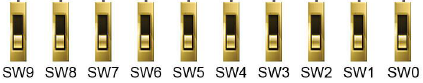
\includegraphics{slide_switch_shorthand.PNG}
    \caption{Display of the slide switches and their appropriate labels \cite{soc_manual}.}
    \label{fig:slide_switch_shorthand}
\end{figure}

\subsection{Buttons}
There are two buttons which impact the functionality of the board. KEY3 is the \textbf{action button}. It is the button you hit to set values, and will be referred to as the \textit{action button} from now on. KEY0 is the \textbf{reset button}. While encoding or decoding values using the enigma machine, you can reset the rotors to the daily settings by hitting this button. More details on this will become clear in the following sections. This button will be referred to as the \textit{reset button} from now on. 

They were placed far apart to avoid accidentally hitting the wrong button. Accidentally depressing the reset button would require the user to restart the message encoding / decoding procedure entirely, which is not something that we want to have happen. 

\subsection{Operation Mode}
Let's briefly ignore the various setup tools made available to us and use the default settings to get a good idea of how the operation of the Enigma works. In order to get into operation mode, all you need to do is make sure that \textbf{SW9} (or the \textit{setup\_switch}) is down. You will know you are in operation mode if \textbf{HEX5} (the left most display) is displaying the letter O. 

\subsubsection{Operation Displays}
In operation mode \textbf{HEX1} indicates the current letter that you have selected by your input switches (refer to table \ref{tab:gen_switch_func} for indication of what these switches are). \textbf{HEX0} indicates the current translation of your input value by the enigma machine. \textbf{The general procedure for encoding a message is the following: }
\begin{itemize}
    \item Push and release the reset button.
    \item Set the input switches to the value you want to input, which you can verify in \textbf{HEX1}.
    \item Push and release the action button. You will notice that HEX0 will change when you press the action button. Note that it does not necessarily need to change though. 
    \item The encoded letter for your input is the letter in HEX0. Write down HEX0. 
    \item Repeat steps 2 through 5 until you have completed your message. 
\end{itemize}


\textbf{Likewise the decoding procedure is as following: }

\begin{itemize}
    \item Push and release the reset button.
    \item Set the input switches to the value you want to decode, which you can verify in \textbf{HEX1}.
    \item Push and release the action button. You will notice that HEX0 will change when you press the action button. Once again, it doesn't necessarily need to change. 
    \item The decoded letter for your input is the letter in HEX0. Write down HEX0. 
    \item Repeat steps 2 through 5 until you have completed decoding your message. 
\end{itemize}

Note that the above procedure assumes that the enigma you are encoding and decoding with are set to the same \textit{initial settings}. We will discuss initial settings later in this guide. 

This is all you need to know as far as the general operation of the enigma is concerned. However, the most important part of the enigma machine's encryption is being able to change the initial setting of the machine. The setup of the machine is discussed in the following sections. 

\subsection{Switches}
Before we can dive into the different setup configurations of the enigma, it is important to understand the switches and their general purpose. There are nine switches on the FPGA, all of which are used to some extent for the user interface of the enigma. They are broken up into four distinct groups as you can see in table \ref{tab:gen_switch_func}. Each of the groups' options and particularities are explained in the appropriate section. 

\begin{table}[ht!]
    \centering
    \begin{tabular}{|c|c|c|}
        \hline
        Group & Switches & Functionality \\
        \hline \hline
        Setup& \small{SW9} & \footnotesize{Toggles between setup and operation mode} \\
        \hline
        Setup Type & \small{SW8 \& SW7} & \footnotesize{Allows us to select what we are setting up (4 options)} \\
        \hline
        Setup Side & \small{SW6 \& SW5} & \footnotesize{Allows us to select which side we are setting up} \\
        \hline
        Input Value & \small{SW4-SW0} & \footnotesize{Allows us to input values between 0 and 31} \\
        \hline
    \end{tabular}
    \caption{Description of the switches on the board and their functionality.}
    \label{tab:gen_switch_func}
\end{table}

\subsection{Configuration}
There are four different settings of the enigma, each of which have multiple possible options. The following section explains each of these settings and their possible values, as well as how to set them up. First thing is first, to get into setup mode, put the setup switch high (SW9). Tables \ref{tab:setup_types} and 


\begin{table}[ht!]
    \centering
    \begin{tabular}{|c|c|c|c|}
        \hline
        Setup Type & SW8 & SW7 & Displays \\
        \hline \hline
        Reflector & 0 & 0 & RF \\
        \hline
        Rotor Type & 0 & 1 & RT \\
        \hline 
        Rotor Initial Positions & 1 & 0 & IP \\
        \hline
        Ring Setting & 1 & 1 & RS \\
        \hline
    \end{tabular}
    \caption{Setup types and their switch configurations.}
    \label{tab:setup_types}
\end{table}


\begin{table}[ht!]
    \centering
    \begin{tabular}{|c|c|c|c|}
        \hline
        Setup Side & SW6 & SW5 & Displays \\ 
        \hline \hline
        Right & 0 & 0 & R \\
        \hline
        Middle & 0 & 1 & M \\
        \hline
        Left & 1 & D & L \\
        \hline
    \end{tabular}
    \caption{Setup sides and their switch configurations.}
    \label{tab:setup_sides}
\end{table}

\subsubsection{Reflector}
In the chain of scrambling of the enigma, the reflector scrambles the forward going path and send it back on its way down the reverse path. From the users perspective there are two possible values that the reflector can be set to (i.e. two mappings from the forward output to the reverse input). In order to set the reflector, you need to have both of the \textit{setup type} switches down (SW8 and SW7). You will know you are setting up the correct setting if HEX3 and HEX2 read `RF'. In this state, you can see the current value of the reflector (0 or 1) in HEX0. You can use SW0 to choose a value for the reflector (which you can verify in HEX1) and you can set the reflector value by pushing the action button. 

\subsubsection{Rotor Type}
Each rotor (there are three) has a mapping from one letter to another (or in some cases itself). These mappings are what scramble the input code. There are four different possible mappings for each rotor of this particular enigma machine. In order to set a particular rotor's type, we must get into the `rotor type' setup mode, and we must select the appropriate rotor (right, middle, left) at which point we can set the particular value. 

Refer to table \ref{tab:setup_types} in order to see where to set switches 7 and 8 to get into \textit{Rotor Type} mode. From there you can pick which side you want to set using switches 5 and 6 (consult table \ref{tab:setup_sides} to see how to pick a particular side). Once you have picked a side, HEX0 will show the current rotor type of that side. You can adjust the value sliders (SW4-SW0) to pick a rotor type value between 1 and 4. The current value being interpreted based on your inputs is displayed in HEX1. Set the value to what you want and press the action button to set the rotor type to the value you have selected. 


\subsubsection{Rotor Initial Positions}
If each rotor started at the same point every time we encrypted a message, the encryption wouldn't be very difficult to crack at all. Luckily for us, we are able to start each of the three rotors at any of 26 initial positions, we can even change them on the fly using agreed upon techniques if both the person encoding the message and the person decoding the message know how to follow along. 

Again refer to table \ref{tab:setup_types} in order to see where to set switches 7 and 8 to get into \textit{Rotor Initial Positions} mode. From there you can once again pick which side you want to set using switches 5 and 6. HEX0 will show the current starting letter (initial position) of the particular rotor and HEX1 will display the currently selected value of the input slide switches (SW4-SW0). Once you have picked the value that you would like, you may press the action button and you will set the rotor initial position. 

\subsubsection{Ring Setting}
On top of the initial positions of the rotors, we have an initial scrambling step called the ring setting. There is a particular ring setting for each of the three rotors and each ring setting can be set independently. 

Once again, refer to table \ref{tab:setup_types} in order to see where to set switches 7 and 8 to get into \textit{Ring Setting} mode. From there you can once again pick which side you want to set using switches 5 and 6. HEX0 will show the current ring setting (a letter between A - Z symbolizing the shift) of the particular rotor and HEX1 will display the currently selected value of the input slide switches (SW4-SW0). Once you have picked the value that you would like, you may press the action button and you will set the ring setting for the particular rotor.

\clearpage

\bibliographystyle{unsrt}
\bibliography{bibliography}

\end{document}
